\chapter{An Implicit Probabilistic Generative Model}
\label{chapter8}
\graphicspath{{source/chapter8/}}
In previous chapters, we discussed learning in both undirected (Chapter~\ref{chpt5:undirecteLearning}) and directed (Chapter~\ref{chpt6:em-flow} and \ref{chpt7:genhmm}) graphical models. In previous discussion, model learning has been mainly based on the maximum likelihood principle, which includes the cases of MRF learning with approximate inference and the likelihood variational lower bound such as \eqref{chpt5:eq:lower-bound-F}. With maximum likelihood learning, if the exact likelihood is not available, its variational or approximate value is usually used as the objective function.

In this chapter, we introduce a way of learning a generative model that does not use maximum likelihood. Different from distributions induced by normalizing flows in previous chapters, we do not require the induced distribution $p(\bm{x};\bm{\theta})$ by a generator in the generative model to be tractable here. In other words, the generator-induced distribution $p(\bm{x};\bm{\theta})$ is \textit{implicit} and likelihood-intractable. This relaxation indeed gives us larger freedom of defining the generators since we do not track the Jacobian computation anymore, and thus enlarges the hypothesis space of the model distribution $p(\bm{x};\bm{\theta})$. But it also brings the question of how to learn such a model without the tractable density function, since maximum likelihood and its associated KL divergence require evaluation of likelihood according to explicit probability density (mass) functions.  Perhaps, a question before the \textit{how} is the \textit{why}, i.e., why do we need such kind of probabilistic models?

The motivation for studying these generative models lies in applications where sampling from implicit distributions is more important than likelihood tractability. In high-dimensional spaces, deep generative models that are defined with neural network based generators and induce implicit distributions, demonstrate their advantage in the efficiency of modeling complex distributions and sampling, in comparison with explicit statistic models. This allows the representation and manipulation of implicitly high-dimensional distributions via the generative models. For instance, deep generative models have been used in image super-resolution, image-to-image translation, speech synthesis, etc. Besides, implicit generative models can be naturally incorporated in reinforcement learning where typically an agent tries to learn to finish some tasks via interacting with a dynamic environment. For instance, in model-based methods, using a generative model to represent the environment and generating states for the agent to learn with, offers the way of training agents in simulations. A policy, essentially a conditional distribution of actions given an environment state, may be modeled by an implicit generative model since we mainly need to get the action in the current environment.

In this chapter, we introduce the learning of implicit probabilistic generative models by employing \textit{optimal transport} from transportation theory that does not need the tractability of likelihood. As long as we can sample from a generative model efficiently, learning of the generative model can be formed as the minimization of an optimal transport distance between the induced implicit distribution and an empirical distribution.

\section{Optimal Transport}\label{chpt8:sec:ot}
Optimal transport (OT) is a geometric tool for comparison of probability distributions, which has a rich history. Its work traces back as early as $18$th century in Monge's work \cite{monge1781memoire}. OT has been widely used in different fields, such as economic problems, logistics, production planning, etc. Along with its development in history, OT has been given different names, such as earth mover distance, Kantorovich distance, and Wasserstein distance. Abstractly, OT distance measures the minimum transportation cost of moving the mass of a distribution to another distribution \cite{villani2003topics}. Due to its close relation to the comparison of probability distributions and optimization, OT and its
variants have also been popularly used in machine learning and gained fast development in both theory and applications \cite{2013arXiv1310.4375C, 2013arXiv1306.0895C, 2016arXiv161006519S, ClaiciCS18}.

The high-level idea of this chapter is to use the OT distance to guide us to find the distribution $p(\bm{x}; \bm{\theta})$ of a generative model to approximate the true distribution $p^{\ast}(\bm{x})$. We begin with the introduction to OT itself and make connections to some popular generative models.

We denote the space $(\bm{\Xx},\|\cdot\|_2)$ be our working space, where $\bm{\Xx} = \prod_{x=1}^{N} \Xx_i$ as defined in Chapter~\ref{chapter2}. $\|\cdot\|_2$ is the Euclidean distance. Different from the discussion on learning in Section~\ref{chpt2:sec:learning-principles} and \ref{chpt5:sec:futher-dis-learning}, we explore the model learning without requiring the likelihood of probabilistic models.
 Assume that $\bm{\Xx}_1$, $\bm{\Xx}_2$ are finite sample subsets of $\bm{\Xx}$. Let $p^{\ast}(\bm{x})$ be a distribution on $\bm{\Xx}_1$ and $p(\bm{x};\bm{\theta})$ be a distribution on $\bm{\Xx}_2$.
With mild abuse of notation, we denote the OT distance between $p^{\ast}(\bm{x})$ and $p(\bm{x}; \bm{\theta})$ by $T(p^{\ast},p)$. According to Kantorovich's transportation problem\cite{villani2003topics}, we have $T(p^{\ast},p)$ given by
\begin{equation}\label{chpt8:eq:ot}
  T(p^{\ast}, p) = \min_{\pi\in\Pi(p^{\ast}, p)}\langle\pi,\bm{M}\rangle,
\end{equation}
where $\dotp{\cdot}{\cdot}$ stands for the Frobenius inner product of
two matrices, and $\Pi(p^{\ast},p)$ is a set of joint distributions $\pi$ on
the sample sets $\bm{\Xx}_1\times\bm{\Xx}_2$ such that $\pi$ has
marginal distributions $p^{\ast}(\bm{x})$ and $p(\bm{x}; \bm{\theta})$. 
The cost matrix $\bm{M}$ has elements $M_{i,j} = d(\bm{x}_1^{i}, \bm{x}_2^{j})$ with $d(\cdot, \cdot)$ as a distance (Euclidean distance is used in our implementation), where $\bm{x}_1^{i}\in\bm{\Xx}_1$ and $\bm{x}_2^{j}\in \bm{\Xx}_2$ are $i$th and $j$th samples from $p^{\ast}(\bm{x})$ and $p(\bm{x}; \bm{\theta})$, respectively. 


\begin{remark}[Connection to the vanilla generative adversarial network]
  In the model learning of previous chapters, the information on how the model should adjust (change its parameter) is given by the likelihood value (and its gradients), stemming from KL divergence. In this chapter, we introduce the OT distance to offer such information in modeling learning. There are other ways to achieve this goal. A popular one is the generative adversarial network (GAN) \cite{goodfellow2014gan, 2017arXiv170100160G}, which casts the generative model learning into an adversarial game between the generator $\bm{g}$ and a discriminator $f$.
The {discriminator} $f$ gets input from either output of $\bm{g}$ or from
$p^{\ast}$. The generator $\bm{g}$ and discriminator ${f}$ play against each other
regarding a min-max objective
\begin{equation}\label{chpt8:eq:eq-gan}
  \min_{\bm{g}} \max_f \EE_{p^{\ast}(\bm{x})}\left[ \log(f(\bm{x})) \right] + \EE_{p(\bm{z})}\left[ \log(1-f(\bm{g}(\bm{z})) \right],
\end{equation}
where $p(\bm{z})$ is a fixed distribution and easy to sample from. The model distribution $p(\bm{x}; \bm{\theta})$ is an implicit distribution and is induced by $\bm{x} = \bm{g}(\bm{z})$.
The probabilistic model learning relies on if min-max game finds
its equilibrium where distribution $p(\bm{x}; \bm{\theta})$ is the same as $p^{\ast}(\bm{x})$ and
$f$ is optimal. In optimal case of the discriminator, objective of
\eqref{chpt8:eq:eq-gan} is equivalent to minimize the Jensen-Shannon divergence between $p(\bm{x}; \bm{\theta})$ and $p^{\ast}(\bm{x})$.
\end{remark}


\begin{remark}[Connection to Wassertein GAN]\label{chpt8:rmk:wgan}
  It is interesting to note that the OT minimization can be connected to GANs via its duality form. According to Kantorovich-Rubinstein duality \cite[Section~2.4]{2018arXiv180300567P}\cite{villani2008optimal},
  \begin{equation}\label{chpt8:eq:kr-duality}
     T(p^{\ast},p) = \sup_{\|f\|_{L} \leq 1} \EE_{p^{\ast}(\bm{x})}\left[ f(\bm{x}) \right] -
  \EE_{p(\bm{x};\bm{\theta})}\left[ f(\bm{x}) \right],
\end{equation}
$\|f\|_L$ is a constraint for $f$ such that $f$ belongs to the 1-Lipschitz function
family. That is to say, $f$ in \eqref{chpt8:eq:kr-duality} can be any function from the 1-Lipschitz function
family (which is different from the binary discriminator in \eqref{chpt8:eq:eq-gan}) that maximizes the objective in \eqref{chpt8:eq:kr-duality}. Then minimization of the OT distance is formulated as a min-max problem \cite{2017arXiv170107875A}, termed as Wasserstein GAN (WGAN),
\begin{equation}\label{chpt8:eq:eq-wgan}
  \min_{\bm{g}} \max_{\|f\|_{L} \leq 1} \EE_{\bm{x} \sim p^{\ast}(\bm{x})}\left[ f(\bm{x}) \right] -
  \EE_{\bm{z}\sim p(\bm{z})}\left[ f(\bm{g}(\bm{z})) \right],
\end{equation}
where $p(\bm{x};\bm{\theta}) = p(\bm{g}(\bm{z}); \bm{\theta})$ with $\bm{\theta}$ parameterizing $\bm{g}$ and $\bm{z}\sim p(\bm{z})$. The Lipschitz constraint enforcing is not trivial in general, especially for the deep generative models where $\bm{g}$ is implemented by neural networks.
The similarity between the vanilla GAN in \eqref{chpt8:eq:eq-gan} and the dual problem in \eqref{chpt8:eq:eq-wgan} can be seen from both their problem definitions and interpretations. Firstly, they are both min-max adversarial games between a generator $\bm{g}$ and a score function $f$. Secondly, in both cases, $\bm{g}$ tries to increase the scores of its generated samples $f(\bm{g}(\bm{z}))$, while the score function $f$ tries to increase the scores of true samples and to decrease the scores of generated samples at the same time.
\end{remark}

\begin{remark}[Connection to auto-encoders]
It is known that the variational lower bound of the likelihood function as in \eqref{chpt5:eq:lower-bound-F} is used to train variational auto-encoders, where an encoder and a decoder adjust their parameters to maximize the variational lower bound in the maximum likelihood principle. Since OT offers an alternative tool for modeling learning, it is also employed to train auto-encoders in likelihood-free settings, which shares similarities with the variational auto-encoders. See \cite{patrini2018sinkhornVAE, genevay2017gan,bousquet2017optimal, ambrogioni2018wasserstein} for detailed discussions.
\end{remark}

\section{EOT based Generative Models}

The optimal transport problem in \eqref{chpt8:eq:ot} is highly intractable. Therefore, approximation has to be used for efficient solutions. In Remark~\ref{chpt8:rmk:wgan}, Kantorovich-Rubinstein duality offers one way to solve the problem in its dual form if the Lipschitz constraint can be properly enforced. An alternative way can be by using entropy regulation to seek for a \textit{soft} solution. In this section, we introduce the entropy-regularized optimal transport (EOT) cost and then propose generative models accordingly.

\subsection{Entropy-regularized OT} 

OT calculates the minimum cost of transporting distribution $p^{\ast}(\bm{x})$ to $p(\bm{x}; \bm{\theta})$. We use $W(p^{\ast},p)$ to denote entropy-regularized OT (EOT) cost as follows:
\begin{equation}\label{eq-entropic-wsd}
  W(p^{\ast},p)=\min_{ \pi \in \Pi(p^{\ast}, p)} \dotp{\pi}{\bm{M}} - \la H(\pi),
\end{equation}
where $H(\pi)$ is the entropy of joint distribution $\pi$, i.e., $H(\pi) = \sum_{i,j} -\pi_{i,j}
\log(\pi_{i,j})$ and $\la \in \RR_{+}$ is the regularization
parameter. Here $\RR_{+}$ denotes positive scalars. The entropy regularization in \eqref{eq-entropic-wsd}  translates 
to a requirement that the joint distribution $\pi$ has a high entropy. 
 The duality of EOT cost in \eqref{eq-entropic-wsd} is
\begin{equation}\label{eq-dual-wsd}
  W(p^{\ast}, p)  =  \max_{\bm{\al}, \bm{\be} \in \mathbb{R}^{N}} \bm{\al}^{\intercal}p^{\ast} + \bm{\beta}^{\intercal}p \! - \!
  \sum_{i,j} \lambda e^{ \frac{{\left( \al_i + \beta_j - M_{i,j} \right)}}{\la} },\vspace{-2pt}
\end{equation}
where $\bm{\alpha},\bm{\beta}$ are dual variables, $(\cdot)^{\intercal}$ means transpose, $\alpha_i$ is the $i$th element of $\bm{\alpha}$, and $\beta_i$ is the $j$th element of $\bm{\beta}$.

One benefit of having the dual variables in this form is that the optimal dual vector $\bm{\beta}^{\ast}$
of \eqref{eq-dual-wsd} is a subgradient of $W(p^{\ast},p)$ with respect to $p$. Thus, if we can efficiently obtain the optimal dual vector $\bm{\beta}^{\ast}$, we can learn our model distribution $p(\bm{x}; \bm{\theta})$ via the subgradient $\bm{\beta}^{\ast}$.

There is a computationally efficient algorithm called Sinkhorn
algorithm\cite{2013arXiv1306.0895C, 2013arXiv1310.4375C} to
solve~\eqref{eq-dual-wsd}, which alternatively scales the rows and columns of matrix $e^{-\frac{\bm{M}}{\lambda}}$. This alternative computation gives a pair of vectors $(\bm{u}, \bm{v}) \in \RR^N_{+} \times \RR^N_{+}$ that defines the optimal primary and dual variables \cite[Proposition~2]{2013arXiv1310.4375C},
\begin{align}\label{eq-dual-opt}
  \pi^{\ast} &=
               \mathrm{diag}(\bm{u}) \, e^{\frac{-\bm{M}}{\la}} \, \mathrm{diag}(\bm{v}),  \nonumber \\
  \bm{\beta}^{\ast} &= \frac{\log(\bm{u}^{\intercal})\mathds{1}_N}{N\la} \mathds{1}_N -\frac{\log(\bm{u})}{\la}.
\end{align}
where $\mathrm{diag}(\bm{u})$ is a matrix with diagonal entries from vector $\bm{u}$ and $\mathds{1}_N$ is a column vector with ones.


\subsection{Two Generative Models Derived from EOT}

In this section, we propose two generative models.
We first develop an EOT based generative model handling signals/data directly. This model is termed as EOT generative model (EOTGM). 
In our second model, we use a
representation mapping where EOT cost is used to optimize the
generative model and representation mapping jointly. The second model is named as EOT based GAN (EOTGAN).

\subsubsection{EOTGM}\label{subsec-gmeot}
{The true probability distribution $p^{\ast}(\bm{x})$ is not available but its empirical distribution is available, i.e., the dataset. We carry on using the notation $p^{\ast}(\bm{x})$ as the target distribution. $p(\bm{x};\bm{\theta})$ is the probability distribution of our model induced by a generator $\bm{g}: \bm{\Zz} \rightarrow \bm{\Xx}$, where $\bm{\Zz}$ is the support set of latent distribution $p(\bm{z})$. The generator $\bm{g}$ is implemented by a neural network and maps latent signal $\bm{z} \in \bm{\Zz}$ to signal in $\bm{\Xx}$, i.e., $\bm{g}(\bm{z}) \in \bm{\Xx}$. The latent distribution is assumed to be known. The mapped signal $\bm{g}(\bm{z}) \sim p(\bm{x};\bm{\theta})$ since $\bm{g}$ induces the model distribution. Actually, the parameter of $p(\bm{x};\bm{\theta})$ is the parameter of the generator $\bm{g}$. Applying EOT cost to learn $p(\bm{x}; \bm{\theta})$ is equivalent to minimizing $W(p^{\ast}, p)$ with regard to the generator $g$}
\begin{equation}\label{eq-entropic-model}
  \underset{\bm{g}:\bm{\mathcal{Z}}\to \bm{\Xx}}{\argmin}\, W(p^{\ast}, p) = \underset{\bm{\theta}}{\argmin}\, W(p^{\ast}, p).
\end{equation}
Since $\bm{\beta}^{\ast}$ in \eqref{eq-dual-opt} is subgradient of $W(p^{\ast}, p)$ with regard to $p(\bm{x};\bm{\theta})$, we are able to
optimize the generator $\bm{g}$ such that the induced distribution $p(\bm{x};\bm{\theta})$ approximates $p^{\ast}(\bm{x})$, using gradient chain rule gives
\begin{equation}
  \nabla_{\bm{\theta}}W(p^{\ast}, p) = \left(\nabla_{\bm{\theta}}p\right)^{T} \bm{\beta}^{\ast}.
\end{equation}
Alternatively the optimization problem \eqref{eq-entropic-model} can be addressed by solving $\argmin_{g}\dotp{\pi^{\ast}}{\bm{M}} $ iteratively using auto-gradient functions in PyTorch\cite{pytorch} or
TensorFlow\cite{tensorflow}, where $\pi^{\ast}$ is the solution to the primary problem \eqref{eq-entropic-wsd} given by \eqref{eq-dual-opt}. We
propose Algorithm~\ref{algo-E-WL} to learn distribution $p^{\ast}$
via minimizing the EOT loss with regard to parameter $\bm{\th}$ of generator function $\bm{g}$.
\begin{algorithm}[!tp]
  \caption{EOT based Generative Model (EOTGM)}\label{algo-E-WL}
  \begin{algorithmic}[1]
    \STATE{$l$: the update rate at each iteration. $N$: the batch
      size. $\bm{\th}_{0}$: the initial parameter for $\bm{g}$.}
    \WHILE{$\bm{\theta}$ has not converged}
    \STATE Sample  a batch from a real dataset, $\left\{ \bm{x}^{i} \right\}_{i=1}^{N} \sim p^{\ast}$. 
    \STATE Sample $\left\{ \bm{z}^{i} \right\}_{i=1}^{N} \sim p(\bm{z})$, a batch of latent samples.
    \STATE Pass $\left\{ \bm{z}^{i} \right\}_{i=1}^{N}$ through the generator $\bm{g}$.
    \STATE Calculate the cost matrix $\bm{M}$.
    \STATE $\pi^{\ast}$, $\bm{\beta}^{\ast} \gets$ primary and dual
    solutions of $W(\left\{ \bm{x}^{i} \right\}_{i=1}^{N}, \left\{
      \bm{g}(\bm{z}^{i})\right\}_{i=1}^{N})$ according \eqref{eq-dual-opt}.
    \STATE $\bm{\theta} \gets \bm{\theta} - l \left(\nabla_{\bm{\th}}{p}\right)^{\intercal}
    \bm{\beta}^{\ast}$, or back propagation using loss $\dotp{\pi^{\ast}}{\bm{M}}$
    \ENDWHILE
  \end{algorithmic}
\end{algorithm}

\subsubsection{EOTGAN}

In this section, we consider representation learning (i.e., feature
learning) with which the usage of EOT is more meaningful than that
directly in signal space $\bm{\Xx}$.
It is well-known that Euclidean distance is not well suited to compare
two multimedia signals. For example, Euclidean distance between an
image and its rotated version can be large, but they are visually the same. In Algorithm \ref{algo-E-WL} we construct the cost matrix $\bm{M}$ in EOT using 
Euclidean distance between real signals and generated signals. Our new proposal is to transform a signal through a representation mapping 
$\bm{f}: \bm{\Xx} \rightarrow \bm{\Mm}$, $\bm{\mathcal{M}}\subset\mathbb{R}^{m}$, and we compare features in the representation space via EOT. We assume that Euclidean distance
between features in the representation space is more semantically
meaningful. An element of the cost matrix $\bm{M_f}$ in representation domain (feature domain) is
\begin{equation}\label{def-similarity}
  d_{\bm{f}}(\bm{x}, \bm{y}) = \|\bm{f}(\bm{x})-\bm{f}(\bm{y})\|_{2}.
\end{equation}

Our new objective is joint learning of generator $\bm{g}$ and representation $\bm{f}$. A natural question is how to construct the function $\bm{f}$? {Inspired by the triplet loss in \cite{7298682} aiming at larger distance between distinct classes than in-class distance, we may consider two virtual classes labeled by $p^{\ast}(\bm{x})$ and $p(\bm{x};\bm{\theta})$.
This means that the representation function $\bm{f}$ should have the algebraic property: $ d_{\bm{f}}(\bm{x}_1, \tilde{\bm{x}}_1) + \gamma \leq d_{\bm{f}}(\bm{x}_1, \bm{x}_2) $ for $\gamma > 0$, where $\bm{x}_1, \tilde{\bm{x}}_1 \in \bm{\Xx}_1$ are two samples from distribution $p^{\ast}$ and $\bm{x}_2$ is a generated signal from distribution $p(\bm{x};\bm{\theta})$, i.e., an output of $\bm{g}$. Meanwhile, $\bm{g}$ tries to mitigate this distinction.}

Following the above idea, we do the learning of mapping $\bm{f}$ and generator $\bm{g}$ in $\bm{\Mm}$. Samples from $p^{\ast}(\bm{x})$ and $p(\bm{x}; \bm{\theta})$ are mapped by $\bm{f}$ before we use EOT to measure their similarity.
Let us denote the mapped distributions via $\bm{f}$ by $p^{\ast}_{\bm{f}}$ and $p_{\bm{f}}$, respectively. Let $\bm{M}_{\bm{f}}$ be the cost matrix in representation domain and its elements $M_{\bm{f},{i,j}} = d_{\bm{f}}(\bm{x}^{i}_1, \bm{x}^{j}_2)$, $\bm{x}^{i} \sim p^{\ast}(\bm{x}), \bm{x}^{j}\sim p(\bm{x}; \bm{\theta})$. Then we learn $\bm{f}$ and $\bm{g}$ using alternative optimization, as follows. 
\begin{itemize}
\item Learning of representation $f$ via minimization of the EOT cost
  \begin{equation}\label{eq-sim-in}
    W(p^{\ast}_{\bm{f}},p^{\ast}_{\bm{f}}) = \min_{\widetilde{\pi} \in \Pi(p^{\ast}_{\bm{f}}, p^{\ast}_{\bm{f}}) } \dotp{\widetilde{\pi}}{\widetilde{\bm{M}}_{\bm{f}}} - \la H(\widetilde{\pi}),
  \end{equation}
  where $\widetilde{M}_{\bm{f}, {i,j}} = d_{\bm{f}}(\bm{x}^{i}, \tilde{\bm{x}}^{j})$, $\bm{x}^{i}, \tilde{\bm{x}}^{j} \sim p^{\ast}(\bm{x})$, and maximization of the EOT cost
  \begin{equation}\label{eq-sim-ex}
    W(p^{\ast}_{\bm{f}}, p_{\bm{f}}) = \min_{{\pi} \in \Pi(p^{\ast}_{\bm{f}}, p_{\bm{f}}) } \dotp{{\pi}}{\bm{M_f}} - \la H({\pi}).\vspace{-8pt}
  \end{equation}
\item Learning of generator $\bm{g}$ via minimization of the EOT cost in \eqref{eq-sim-ex}, i.e.,
  \begin{equation}
    W(p^{\ast}_{\bm{f}}, p_{\bm{f}}).
  \end{equation}
\end{itemize} 
Both $W(p^{\ast}_{\bm{f}}, p^{\ast}_{\bm{f}})$ and $W(p^{\ast}_{\bm{f}}, p_{\bm{f}})$ have lower bounds, but no upper bounds. 
We combine the step 1 above using a hinge loss and define the following costs,
\begin{equation}
  \begin{array}{rl}
    &\Ll_{\bm{f}}(p^{\ast}_{\bm{f}}, p_{\bm{f}}) := \max\left(0, W(p^{\ast}_{\bm{f}}, p^{\ast}_{\bm{f}})- W(p^{\ast}_{\bm{f}}, p_{\bm{f}}) \hspace{-2pt}+\hspace{-2pt} \gamma \right),\\
    &\Ll_{\bm{g}}(p^{\ast}_{\bm{f}}, p_{\bm{f}}) := W(p^{\ast}_{\bm{f}}, p_{\bm{f}}),
  \end{array}
\end{equation}
where $\gamma>0$. Hinge loss helps to balance the adversarial training of the $\bm{f}$ and $\bm{g}$.
Note that our hinge adversarial loss shares similarity only in form to the self-attention GAN\cite{2018arXiv180508318Z} and geometric GAN\cite{2017arXiv170502894L} but is motivated differently and defined in a different metric. We use neural networks for constructing the $\bm{f}$ and $\bm{g}$ functions. Let us assume that the parameters of $\bm{f}$ and $\bm{g}$ are $\bm{\omega}$ and $\bm{\theta}$, respectively. Then the adversarial training between representation $\bm{f}$ and
generator $\bm{g}$ is the following alternating optimization problem
\begin{equation}
  \begin{array}{rl}
    &\min_{\bm{f}} \Ll_{\bm{f}}(p^{\ast}_{\bm{f}}, p_{\bm{f}}) = \min_{\bm{\omega}} \Ll_{\bm{f}}(p^{\ast}_{\bm{f}}, p_{\bm{f}}), \\ 
    &\min_{\bm{g}}\Ll_{\bm{g}}(p^{\ast}_{\bm{f}}, p_{\bm{f}}) = \min_{\bm{\th}}\Ll_{\bm{g}}(p^{\ast}_{\bm{f}}, p_{\bm{f}}).
  \end{array}\vspace{-2pt}
\end{equation}
The algorithm steps of EOTGAN are shown in Algorithm \ref{algo-eWGAN}.
\begin{remark}[Discussion on OT and EOT]

The usage of the entropy regularization in EOT avoids the need for Kantorovich-Rubinstein duality
of OT, thus, is free from the Lipschitz constraint. In the literature, several methods endeavor to
satisfy Lipschitz constraint, for example, projecting neural network
parameters into a space fulfilling Lipschitz constraint via weight
clipping \cite{2017arXiv170107875A}, spectrum
normalization \cite{2018arXiv180205957M}, or adding gradient 
penalty into GAN's cost function \cite{2017arXiv170400028G}. Projecting
approaches bring the problem of neural network capacity underuse and
limit its ability to learn complex mappings. Gradient penalty approaches take
gradients of each layer's weight parameters of a neural network into
GAN's cost, and thus, computational complexity grows fast as the neural
network gets deeper. 
EOT avoids the above-mentioned problems and also has the benefit of lower
computation complexity. With entropy-regularization and Sinkhorn
algorithm, the computation complexity scales as $\mathcal{O}(N^2)$ \cite{2013arXiv1306.0895C}. 
On the other hand, solving OT cost using interior-point methods has a computational requirement as 
$\mathcal{O}(N^3\log{N})$. 

\end{remark}

\begin{algorithm}[!t]
  \caption{EOT based GAN (EOTGAN)}\label{algo-eWGAN}
  \begin{algorithmic}[1]
    \STATE {$l$: the update rate at each iteration. $N$: the batch
      size. $\bm{\th}_{0}$, $\bm{\omega}_0$: the initial parameters for $\bm{g}$ and $\bm{f}$.}
    \WHILE{$\bm{\theta}$ has not converged}
    \STATE Sample two batches of data $ \left\{ \bm{x}^{i}
    \right\}_{i=1}^{N}, \left\{ \tilde{\bm{x}}^{i} \right\}_{i=1}^{N}  $,
    and latent samples $\left\{ \bm{z}^{i} \right\}_{i=1}^{N} $,
    $\bm{x}^{i},\tilde{\bm{x}}^{i} \sim p^{\ast}(\bm{x}), \bm{z}\sim p(\bm{z})$.
    \STATE Pass
    $\left\{ \bm{z}^{i} \right\}_{i=1}^{N}$ through $\bm{g}$.
    \STATE $\widetilde{\pi}^{\ast} \gets$ solve $ W_{\bm{f}}\left( \left\{ \bm{f}(\bm{x}^{i})
      \right\}_{i=1}^{N} , \left\{ \bm{f}(\tilde{\bm{x}}^{i})
      \right\}_{i=1}^{N}\right)$
    \STATE ${\pi}^{\ast} \gets$ solve $W_{\bm{f}}\left( \left\{ \bm{f}(\bm{x}^{i})
      \right\}_{i=1}^{N}, \left\{ \bm{f}(\bm{g}(\bm{z}^i))
      \right\}_{i=1}^{N} \right)$
    \STATE $\partial{\bm{f}} \gets \nabla_{\bm{\om}} \max\left(0,  \dotp{\widetilde{\pi}^{\ast}}{\widetilde{\bm{M}}}-\dotp{{\pi^{\ast}}}{\bm{M}}+ \gamma\right)$
    \STATE $\bm{\om} \gets \bm{\om} - l \cdot \partial{\bm{f}}$
    \STATE Sample $\left\{ \bm{z}^{i} \right\}_{i=1}^{N}$
    and get $ \left\{ \bm{g}(\bm{z}^i)\right\}_{i=1}^{N}$ via $\bm{g}$.
    \STATE $\pi^{\ast} \gets$ solve $W_{\bm{f}}\left( \left\{ \bm{f}(\bm{x}^{i})
      \right\}_{i=1}^{N}, \left\{ \bm{f}(\bm{g}(\bm{z}^{i}))
      \right\}_{i=1}^{N} \right)$
    \STATE $\partial{\bm{g}} \gets \nabla_{\bm{\th}} \dotp{\pi^{\ast}}{\bm{M}}$
    \STATE $\bm{\th} \gets \bm{\th} -l \cdot \partial{\bm{g}}$
    \ENDWHILE
  \end{algorithmic}
\end{algorithm}



\section{Experimental Results}
We perform experiments to verify our arguments on loss choice and algorithms. We evaluate our
generative models on a toy synthetic dataset sampled from a Gaussian-mixture model and the real image dataset MNIST.

\subsection{Evaluation Metrics}\label{subsec-metric}
Similar to Section~\ref{chpt6:sec:eval-metrics}, the Inception Score (IS) \cite{NIPS2016_6125} and Frechet Inception Distance (FID)\cite{2017arXiv170608500H} are used as evaluation metrics of our models. IS is defined as $
  IS(q) = \exp\bigl[ \EE_{\bm{x} \sim q} \mathrm{KL}\bigl( p(c | \bm{x})\| p(c) \bigr)  \bigr]$,
where $\bm{x}\sim q$ indicates synthetic sample from distribution $q$ under testing, $p(c|\bm{x})$ is the conditional distribution of class $c$, and $p(c) = \int_{\bm{x}}p(c|\bm{x})q(\bm{x}) \,d \bm{x} $ is the marginal class distribution computed with $q$. Large IS score means generated samples contain clear objects. Generative models with high IS can output highly diverse samples. Apart from the KL-based metric, an alternative commonly used metric is Frechet Inception Distance (FID)\cite{2017arXiv170608500H}. FID measures the OT distance of two probability distribution by assuming the two distributions are Gaussian, in which case, the closed-form solution is available. Smaller FID means the generated samples are more similar to empirical samples. In short, high IS and low FID are better.


\subsection{Evaluation of EOTGM Using Toy Dataset}\label{subsec-mg}

{We firstly evaluate our proposed EOTGM on a toy dataset sampled from a known probability distribution, a two-dimensional four-mixture Gaussian. This mixture Gaussian is our target distribution to learn, i.e., $p^{\ast}(\bm{x})$. The generator $\bm{g}$ uses a neural network with structure: Input $\rightarrow$ Dense $256$ $\rightarrow$ ReLU $\rightarrow$ Dense $256$ $\rightarrow$ ReLU $\rightarrow$ Dense $256$ $\rightarrow$ ReLU$\rightarrow$Dense $2$. The parameter $\bm{\theta} $ of $\bm{g}$ here is the set of parameters of this neural network. Latent distribution $p(\bm{z})$ used here is standard Gaussian: $\mathsf{N}\left(\bigl(\begin{smallmatrix}& 0\\
    &0\end{smallmatrix}\bigr) ,\bigl( \begin{smallmatrix}1 & 0\\ 0 &
    1\end{smallmatrix}  \bigr)\right)$.
The toy dataset is used by Algorithm~\ref{algo-E-WL} (EOTGM) to train $\bm{g}$. In Figure~\ref{fig-toy}, we plot the empirical samples from our toy dataset and the synthetic samples generated by $\bm{g}$. The corresponding contours are also plotted. It shows that the induced distribution by $\bm{g}$ approaches the mixture Gaussian distribution well without missing any mode.}          

\begin{figure*}[!t]
  \captionsetup[subfigure]{justification=centering}
  \centering
  \begin{subfigure}[b]{0.44\textwidth}
    \centering
    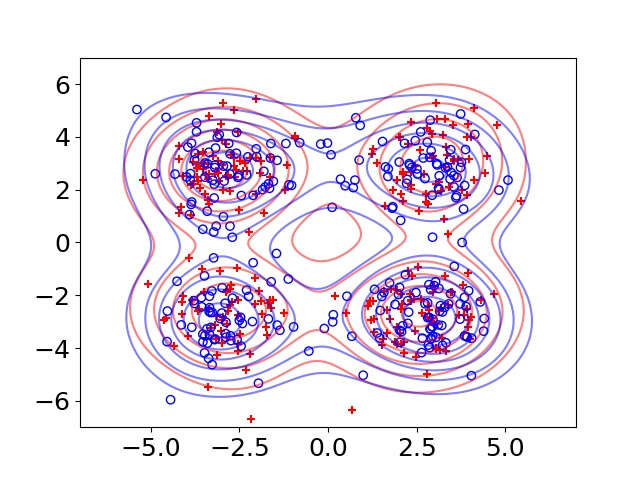
\includegraphics[width=1\linewidth]{images/toy/gauss4/frame8.jpg}
    \caption{}
    \label{fig-toy}
  \end{subfigure}
  \centering
  \begin{subfigure}[b]{0.44\textwidth}
    \centering
    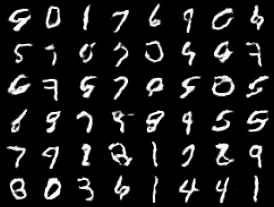
\includegraphics[width=0.85\linewidth]{images/mnist/fake/eot_18500_crop.png}\vspace{5pt}
    \caption{}
    \label{fig-fake-wgan}
  \end{subfigure}
  \caption{Demonstration of sampling. (a) Toy distribution learning ($4$-mixture Gaussians) using EOTGM. Real samples (red '+') and contour
    (red curve), versus generated samples (blue 'o') and contour (blue curve) by $\bm{g}$. (b) Generated samples by EOTGAN for MNIST dataset.}
\end{figure*}


\subsection{Evaluation of Generative Models Using MNIST}
In this section, we evaluate both the generative models using the MNIST dataset.
The representation mapping $\bm{f}$ in EOTGAN adapts two convolutional layers
appended with fully connected layers\footnote{$32$ Conv2d $5 \times5$
  $\rightarrow$ PReLU $\rightarrow$ MaxPool $2\times2$ $\rightarrow$
  $64$ Conv2d $5\times5$ $\rightarrow$ PReLU $\rightarrow$ MaxPool
  $2\times2$ $\rightarrow$ Dense $256$ $\rightarrow$ PReLU
  $\rightarrow$ Dense $256$ $\rightarrow$ PReLU $\rightarrow$ Dense
  $2$}
similar to \cite{1467314}\cite{1640964}. Generator $\bm{g}$ uses the same
setting as that of DCGAN \cite{2015arXiv151106434R} and WGAN \cite{2017arXiv170107875A}. The noise distribution $p(\bm{z})$ is $100$-dimensional standard Gaussian.
We report IS and FID scores of EOTGAN in comparison with DCGAN and WGAN. Since EOTGAN is trained with the representation mapping $\bm{f}$ that
acts as feature mapping, it is not fair to use this representation mapping $\bm{f}$ to do the
evaluation and make comparisons since it would give EOTGAN
advantages. Similar to \cite{2018arXiv180607755X}, we train a
ResNet on MNIST to perform feature extraction for metric measurements
of IS and FID. In addition, we put EOTGM (Algorithm~\ref{algo-E-WL}) in comparison as well.

\begin{figure*}[!t]
  \centering
  \begin{subfigure}[b]{0.44\textwidth}
    \centering
    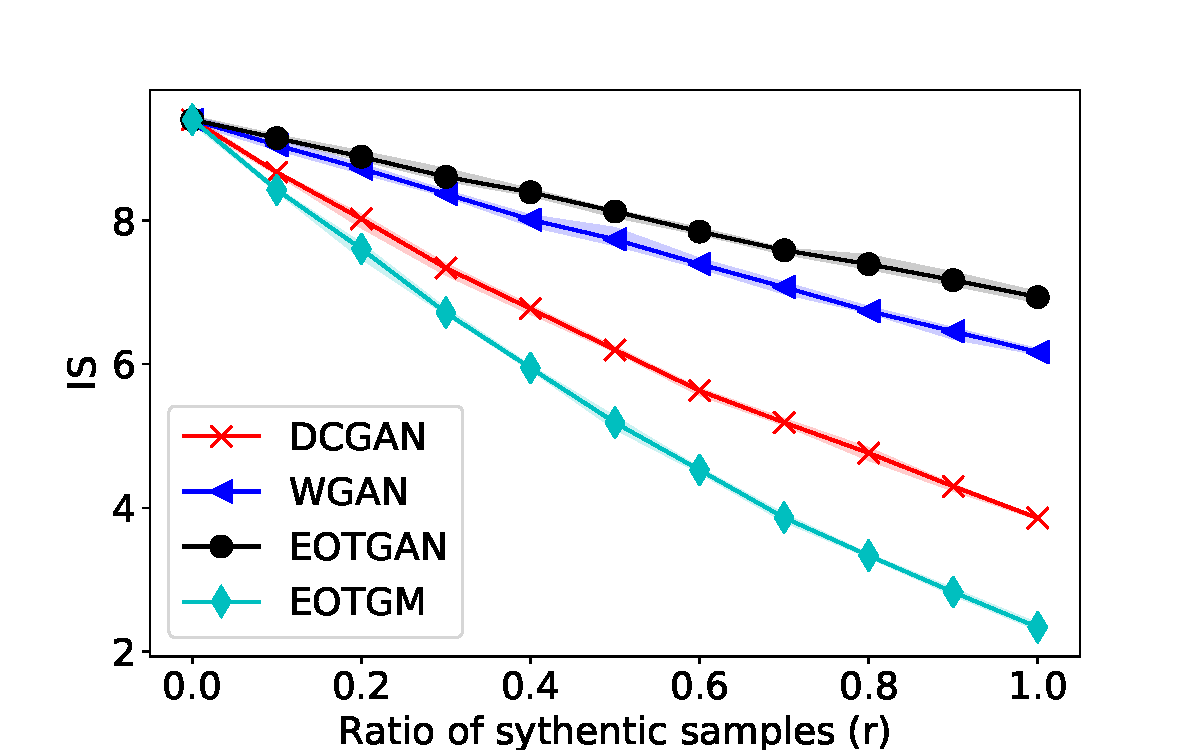
\includegraphics[width=1.1\linewidth]{images/mnist/tra_score/IS_29.pdf}\vspace{-3pt}
    \caption{}
    \label{fig-tra-is}
  \end{subfigure}
  \begin{subfigure}[b]{0.44\textwidth}
    \centering
    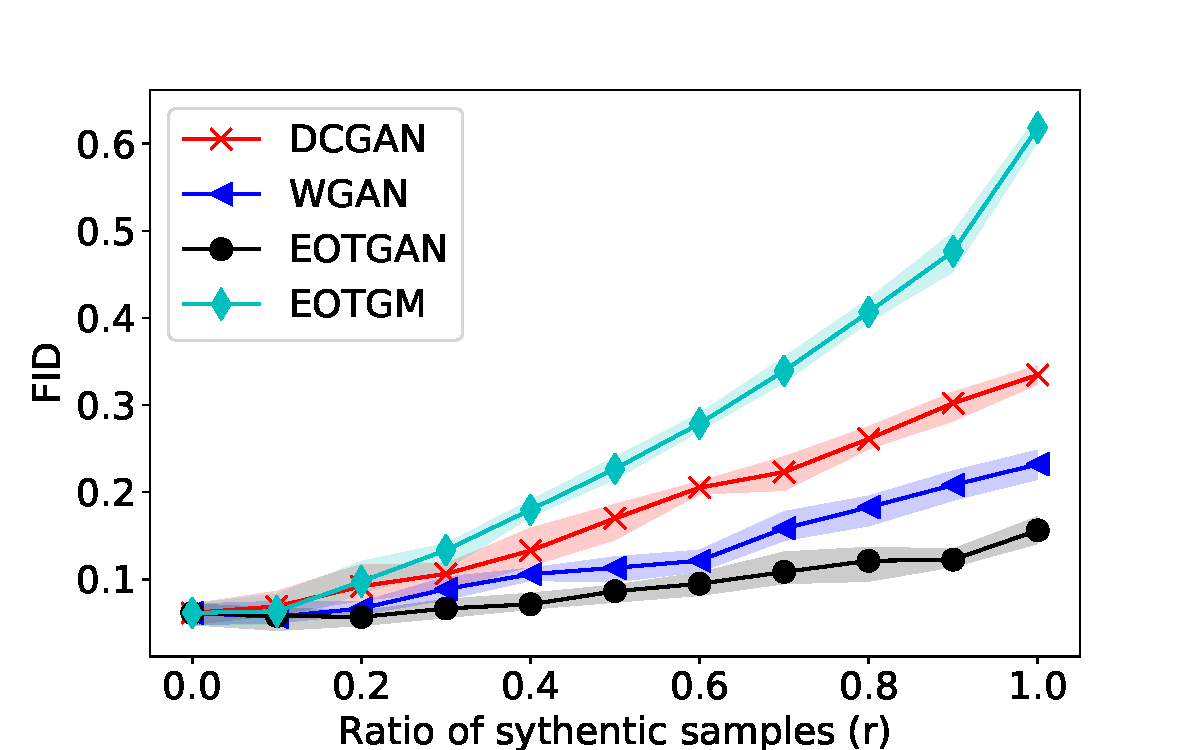
\includegraphics[width=1.1\linewidth]{images/mnist/tra_score/FID_29.pdf}\vspace{-3pt}
    \caption{}
    \label{fig-tra-fid}
  \end{subfigure}
  \caption{Comparison of IS and FID (on MNIST) versus mixing ratio $r$. (For each model at a certain mixture ratio, $5$ experiments are independently performed. Each solid curve with markers plots the mean of $5$ experiments with shaded areas denoting the range of corresponding results.}
  \label{fig-tra-score}
\end{figure*}


Data for evaluations is constructed by mixing empirical samples and
synthetic samples generated by $\bm{g}$. We draw the set $\mathcal{S}_{\mathrm{em}}$ of 2000 empirical samples from MNIST dataset. To generate a set $\mathcal{S}_{\mathrm{syn}}$ of synthetic
samples we draw $2000r$ samples from the generator network $\bm{g}$ where
$r\in[0,1]$ while the remaining $2000(1-r)$ are sampled directly from
MNIST. A demonstration of generated samples from EOTGAN is shown in Figure~\ref{fig-fake-wgan}.
All the following experiments are on
$\mathcal{S}_{\mathrm{em}}$ and $\mathcal{S}_{\mathrm{syn}}$. 
The way of mixing empirical data and generated data helps
us to identify if a metric is intuitively helpful. Among the chosen metrics IS at $r=0$ serves as an upper bound for the test while the FID at $r=0$ serves as a lower bound for the corresponding tests. 

IS measures how certain a classifier assigns a class label to a given
generated sample. The larger IS is, the better the generative model
is. We plot IS versus $r$ for different models in
Figure~\ref{fig-tra-is}. IS scores of all four tested models drop with
an increasing portion of synthetic samples in
$\mathcal{S}_{\mathrm{syn}}$, which is consistent with intuition. IS
of EOTGAN drops at the slowest rate among the four models as more
synthetic samples, for larger $r$, are mixed into test data. It shows
that EOTGAN outperforms WGAN and DCGAN in this test. EOTGM is found to provide the lowest IS.
This may be attributed to the setup that 
EOT optimization with cost measured by Euclidean distance of signals
fails to capture semantic similarity.

In Figure~\ref{fig-tra-fid} the performances of different models are
compared using the FID metric. The smaller the FID of a generative model is, the more similar the
generated samples are to the empirical samples. EOTGAN is the least affected model among all the four, as the ratio $r$ increases, i.e., the generated samples by EOTGAN are more similar to the empirical
ones in the feature space regarding FID. FID of WGAN is larger than that of EOTGAN. As
more generated samples are mixed the FIDs of DCGAN and EOTGM grow
even faster, which means the samples generated by these two models are
less similar to the empirical samples.

\section{Summary}
In this chapter, we took a different approach from previous chapters and considered the learning of implicit probabilistic generative models. An implicit model offers larger freedom in choosing a generator that induces the model distribution, but brings the challenge of model learning due to the loss of tractability of likelihood. Thus optimal transport was introduced and employed to formulate the cost. Optimal transport distance used in learning the model also has interesting connections with generative adversarial networks and auto-encoder-like models. With an entropy-regularization, the optimal transport cost can be computed more efficiently. Two learning algorithms based on the entropy-regularized optimal transport cost were then discussed and demonstrated. 

Different from graphical models discussed in previous chapters, an implicit model has the advantage of flexible generator choice and efficient sampling (or generating sampling). Sampling from an implicit model is usually as simple as a feed-forward operation of the generator once learned. Thus, an implicit model has its application domains where the above-mentioned properties are merited more than explicit form and likelihood tractability of the model's distribution. 


\section{Related Literature}\label{chpt8:sec:literature}

Deep generative models that use non-linear mappings of neural networks have received a lot of attention as a branch of graphical models. The modeling capacity of deep generative models is impressive in high-dimensional spaces (e.g., image super-resolution \cite{ledig2017photo}, image de-noising \cite{CreswellB2017denoise, dilokthanakulmg2016gausian-vae}, image segmentation \cite{marvin2018crf}, speech generation \cite{ryan2018waveglow}, etc.), but the learning of these models is not trivial. The learning difficulty lies in modeling challenges within the high dimensionality or in trading more complex generators (for expressivity) with distribution tractability. Thus, works in pursuit of a better understanding of deep generative models have been carried out, and also different model learning methods and costs have been proposed in relieving the learning difficulty.

One popular track of deep generative models falls into deep variational models which are usually built with the abstraction of graphical models and neural network based generators. To preserve efficient model learning and some level of likelihood tractability, deep generators are usually restricted with special choices of parameterization (e.g., reparameterization \cite{DBLP:journals/corr/KingmaW13}) or generator structures (e.g., the variational inference by normalizing flows, see \cite{rezende2015variational, kingma2016IVF, TomczakW16vae-flow}). These choices of design sometimes also make use of extra auxiliary latent variables in order to further increase the flexibility of generators \cite{ranganath2015hierarchical}. Interesting works falling in this family includes variational auto-encoders (VAEs) \cite{kingma2019vae}, neural variational inference and learning (NVIL) \cite{kuleshov2017neural_variational, mnih14NVIL, Li2020To}, etc. Learning of these models is usually based on the likelihood variational bound (as discussed in Section~\ref{chpt5:sec:futher-dis-learning}) or bounds of this variational bound.

If the generator constraints are further relaxed, more freedom is gained in implementing generators with deep neural networks (which also brings model learning challenges). A prominent example is the generative adversarial network (GAN) \cite{goodfellow2014gan}, which comes with an implicit distribution of the model.
In the vanilla GAN, a generator produces synthetic samples and a discriminator tries to distinguish between real samples and synthetic samples. Generators and discriminators are both implemented using (deep) neural networks, and play an adversary game against each other using a \textit{min-max} optimization to learn parameters of neural networks. More intuitively speaking, for the generator, the game turns out to be minimizing Jensen-Shannon divergence between the target distribution and the induced distribution by the generator when the discriminator is optimal.
This interesting game of casting generative model learning into a adversary game triggered more research in generator and learning method design
\cite{2015arXiv151106434R, 2015arXiv151106434R, 2018arXiv180205957M, 2018arXiv180508318Z, 2018arXiv180600880K, bang2018icml, DBLP:journals/corr/GhoshKNTD17, hoang2018mgan}, and also explanation exploration \cite{2017arXiv170104862A, 2017arXiv170107875A, 2018arXiv180607755X, 2017arXiv170104722M, NIPS2016_6399, li2018graphical}.

Apart from the reasons mentioned above on learning difficulty of deep generative models, new issues raise from the deep generative models themselves. Let us take the learning of the vanilla GAN as an example, which has limitations due to the Jensen-Shannon divergence at the optimal region of its discriminator \cite{2017arXiv170104862A}. Firstly, the limitation is that the gradient of the Jensen-Shannon divergence cost with regard to the generator vanishes as discriminator approaches optimality, which stops the generator from further learning. Secondly, the limitation is due to high sensitivity of Jensen-Shannon divergence to slight perturbations, which can be large between a distribution $p(\bm{x})$ and a distribution $p(\bm{x}+\bm{\epsilon})$ where $\epsilon$ is perturbation. These difficulties were relieved in the followed-up model Wasserstein GAN (WGAN) \cite{2017arXiv170107875A}. Wasserstein distance stems from optimal transport (OT) distance as explained in Section~\ref{chpt8:sec:ot}. The WGAN formulation does not require an explicit discriminator and it does not have the vanishing-gradient issue due to the cost function. Additionally, Wasserstein distance or OT is upper bounded by the standard deviation of perturbation $\epsilon$, addressing the second limitation.

The story did not end there since the duality of Wasserstein distance brought new challenges as discussed in Remark~\ref{chpt8:rmk:wgan}.
Kantorovich-Rubinstein duality used in WGAN requires a supremum over
an infinite set of all Lipschitz functions with Lipschitz constant equal
to one. Various sub-optimal techniques were proposed to enforce the
Lipschitz property. An example was weight clipping
\cite{2017arXiv170107875A} where neural network parameters (weights)
are updated first without Lipschitz constraint and then projected to
satisfy Lipschitz constraint in each iteration. Different enforcement were used later on in addressing it, e.g., gradient penalty\cite{2017arXiv170400028G} and spectrum normalization\cite{2018arXiv180205957M}. Further work attempted OT in different spaces, e.g., \cite{gemici2018primaldual, adler2018banach}.


%%% Local Variables:
%%% mode: latex
%%% TeX-master: "../../main"
%%% End:
